\documentclass[11pt,letterpaper,oneside,openright]{book}

\usepackage[spanish]{babel}
\usepackage[utf8]{inputenc}
\usepackage{lmodern}
\usepackage[T1]{fontenc}

\usepackage{textcomp}
\usepackage[pdftex]{hyperref}
\usepackage{multirow}
\usepackage{booktabs}
\usepackage{graphicx}
\usepackage{tikz}

\usepackage{svg}
\usepackage{amsmath}
\usepackage{listings}
% \usepackage{bordermatrix}
% \usepackage{microtype}
% \usepackage{shortvrb}
% \usepackage{tabularx}
%%%%%%%%%%%%%%%%%
% PARA HACER LA PRUEBA
%%%%%%%%%%%%%%%%%
% \usepackage{nicefrac}
% \usepackage[pdftex]{hyperref}
% \usepackage{anysize}
% \usepackage{fancyhdr}
% \usepackage{subfigure}
% \usepackage{pstricks}
% \usepackage{tabulary}
% \usepackage{type1cm}
% \usepackage{url}
% \usepackage{multirow}
% \usepackage{booktabs}
% \usepackage{subfigure}
% \usepackage{graphicx}
% \usepackage{bm}
%%%%%%%%%%%%%%%%%%%%%%%%%%%%%%%%%%%%%%
% \usepackage[bookmarks]{}
% \usepackage[bookmarks,colorlinks]{hyperref}
\graphicspath{{images/}}
\setsvg{
    svgpath = images/,
    inkscape = inkscape -z -D % conversion options for svg package, export drawing instead of page
}
% \renewcommand{\arraystretch}{1.5}
% \usepackage{hyperref}
\hypersetup{colorlinks,%
            citecolor=black,%
            filecolor=black,%
            linkcolor=black,%
            urlcolor=black}

% \usepackage[charter]{mathdesign}

\title{Desarrollo de una aplicaci\'on móvil para visitas dentro el campus de la UMSS usando Geolocalización}
\author{Edmundo Figueroa Herbas}
\date{\today \ }

\begin{document}
% \include{title-page}
\frontmatter
  \maketitle
  \tableofcontents

\mainmatter{}
  \chapter{Introducción} % (fold)
\label{cha:introduccion}

El presente proyecto consiste en el desarrollo de una aplicación móvil que permita ubicar y encontrar una locación dentro del campus de la Universidad Mayor de San Simón, la aplicación deberá localizar la ubicación actual del usuario y permitir especificar un punto de destino, mostrando a continuación el camino más corto para llegar a destino.

El campus universitario abarca más de 214,000 $m^2$ y encierra varias facultades y oficinas administrativas, para estudiantes nuevos y antiguos o personas que
necesitan hacer trámites administrativos, incluso si solo se quiere conocer el
campus, es necesario contar con un mapa donde ubicarse.

Las aplicaciones móviles tienen una gran demanda por parte de la población ya
que la gran mayoría posee un \emph{smartphone} o teléfono inteligente con capacidad de
ejecutar aplicaciones muy fácilmente, los \emph{smartphones} cuentan también con GPS,
el cual se usa para conocer la ubicación del usuario con un margen de error de
3 metros, usando puntos de referencia geo-localizados se puede determinar la
ruta óptima para llegar a destino. Es una desventaja para nuestra Universidad que no exista información confiable de fácil acceso para poder desplazarse por el campus.

  \section{Antecedentes} % (fold)
  \label{sec:antecedentes}

  Actualmente \emph{Google Maps} ofrece una solución al problema de encontrar una ruta entre 2 puntos geolocalizados, ya que sugiere posibles rutas si se usara movilidad, bicicleta o para ir caminando, para lograr esto se toman en cuenta los distintos tipos de calles que existen y la dirección en el caso de movilidades, \emph{Google Maps} toma en cuenta la descripción de una locación o la referencia cartográfica en latitud y longitud de los puntos, y el cómo se va a desplazar entre los 2 puntos para dibujar con una línea roja la ruta a seguir.

  Así como también existen Blogs o Aplicaciones con información de los lugares turísticos o de interés para visitar en la ciudad, como ser TripAdvisor, la información que provee esta aplicación generalmente incluye la locación del lugar referenciada sobre un mapa estático, este tipo de aplicaciones usa el API de \emph{Google Maps} para lograr encontrar una ruta hacia el lugar de interés.

  En el caso del campus de la Universidad Mayor de San Simón, Google Maps no cuenta con la información para lograr este objetivo, de encontrar una ruta entre 2 puntos geo-referenciados, ya que se necesita de un mapa de los caminos internos del campus Universitario e información de las aulas, kioscos, fotocopiadoras, oficinas, etc. Esta información no está disponible o es de difícil acceso lo cual genera malestar cuando se busca una locación dentro del campus Universitario.

  \section{Descripción del problema} % (fold)
  \label{sec:desc_probl}

  % Al andar dentro del campus universitario buscando algún lugar o punto de interés, es generalmente de gran prioridad reducir el tiempo en el cual se llega al aula u oficina, lamentablemente el campus Universitario carece de un buen sistema de señalización por lo que para llegar al punto de destino es necesario preguntar la  la Universidad hacia gente externa que necesitan hacer uso o encontrar algún lugar en especifico ya que lamentablemente esta información actualmente sólo te la pueden ofrecer las personas que conocen el lugar de antemano y aun en esos casos existe la posibilidad de no encontrar el lugar que se está buscando.\\

  La Universidad Mayor de San Simón no cuenta con un mapa interactivo que
  muestre la ubicación de los puntos o lugares que se encuentran dentro del
  campus universitario y como llegar hasta su ubicación, la falta de señalización obstaculiza el desplazamiento de los estudiantes o personas que requieren encontrar alguna oficina para, por ejemplo, realizar trámites administrativos, encontrar aulas o auditorios, etc. como resultado se pierde tiempo al tratar de encontrarlos por lo que un mapa con estas características sería de gran ayuda para el desplazamiento dentro del campus universitario. En la figura  \ref{fig:arbolProblemas}, se puede apreciar al árbol de problemas.

  % \begin{figure}[!hbp]
  %   \centering
  %   \includesvg{arbolProblemas}
  %   \caption{Diagrama Árbol de Problemas}
  %   \label{fig:arbolProblemas}
  % \end{figure}


  \begin{figure}[H]
    \begin{center}
      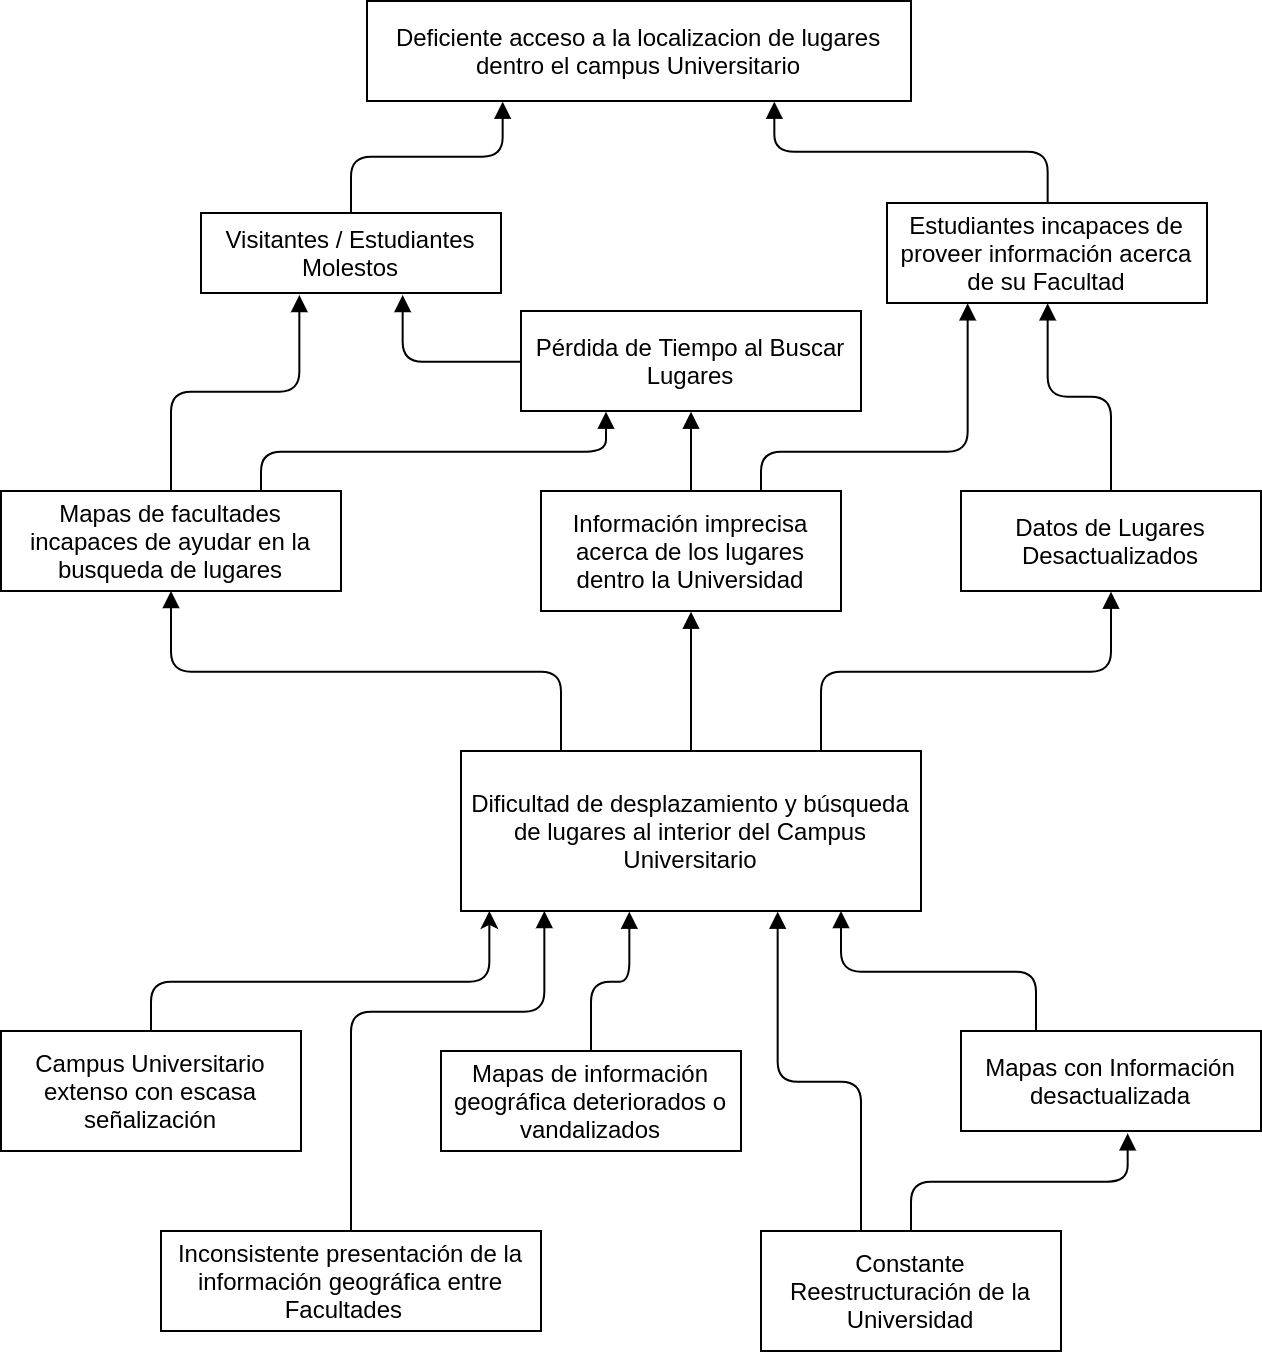
\includegraphics[width=0.65\textwidth]{diagramas/arbolProblemas}
    \end{center}
    \caption{Diagrama Árbol de Problemas}
    \label{fig:arbolProblemas}
    \caption*{Fuente: Elaboración propia}
  \end{figure}

  \section{Objetivo general} % (fold)
  \label{sec:objetivo_general}
    \begin{quote}
      Desarrollar una aplicación web móvil \emph{responsive} para optimizar la búsqueda de lugares y el  desplazamiento al interior del Campus Universitario de la UMSS.
    \end{quote}
  % section objetivo_general (end)


  \section{Objetivos Específicos} % (fold)
  \label{sec:obj_especificos}
    \begin{itemize}
      \item Generar un mapa con información geográfica de las rutas dentro del campus Universitario.
      \item Administrar lugares geolocalizados dentro del campus Universitario.
      \item Mostrar en la aplicación los lugares geolocalizados desplegando la ruta óptima desde mi posición hasta el punto destino.
      \item Administrar usuarios en el sistema.
      \item Registrar las búsquedas sobre rutas realizadas por los usuarios en el sistema.
    \end{itemize}
  % section obj_especificos (end)


  \section{Justificación} % (fold)
  \label{sec:justificacion}

  El Campus Universitario es bastante extenso y se encuentra en constante reestructuración, debido a que las aulas se incrementan, las oficinas son reubicadas, etc. gracias a esto es que los mapas con los que cuenta cada facultad, que son escasos y están impresos sobre banners estáticos, son también difíciles de actualizar. Este hecho genera malestar en estudiantes que llegan tarde a sus clases o necesitan llegar a algún Auditorio o personas/visitantes en proceso de realizar trámites administrativos, no encuentran con facilidad las oficinas a las que necesitan llegar.

  Una aplicación que permita localizar o encontrar locaciones y además proveer la ruta óptima dentro del campus de la Universidad Mayor de San Simón es de gran importancia para brindar apoyo a cualquier persona que necesite desplazarse por el campus Universitario.

  Las Aplicaciones móviles y/o web demostraron ser el futuro del desarrollo de software y la gran mayoría de los países en el mundo consumen estas soluciones y es necesario apuntar a esta tendencia.


  % section justificacion (end)
% chapter introduccion (end)

  \section{Alcance}
  \label{sec:Alcance}

    \subsection{Alcance Práctico}
    \label{sub:alcance_practico}

    Una aplicación web móvil puede llegar a ser muy compleja y manejar información sensible, y ya que el servidor está expuesto al acceso público de los usuarios, es susceptible de ataques maliciosos y malintencionados para acceder y robar información privada que los usuarios podrían tener almacenados en la aplicación, en el caso de la presente aplicación, el sistema no manejará información sensible del usuario, como ser tarjetas de crédito pero la aplicación manejará información de lugares, información que podría ser corrompida por usuarios malintencionados. La seguridad es muy importante para una aplicación web, por lo cual el presente proyecto implementara medidas de seguridad para asegurar la identidad del usuario que está solicitando el ingreso al sistema pero no incluirá protección a ataques Phishing, DoS ya que los objetivos específicos no los contempla.\\


    El \emph{look and feel} de una aplicación web es un tema muy importante para cualquier aplicación a desarrollar, para lograr que la aplicación se muestre de manera consistente en la pantalla de un smartphone se usarán herramientas de terceros pero no se extenderá el uso de la misma para la pantalla de un ordenador de escritorio que posee una resolución de pantalla muy superior al de un celular.\\



    % end alcance_practico

    \subsection{Alcance Metodológico}
    \label{sub:alcance_metodologico}
    Para la conclusión exitosa del presente proyecto se implementará la metodología  Programación Extrema (XP) y cada iteración del proceso tiene como meta el desarrollo conjunto de diferentes módulos, historias de usuario y la documentación relacionada.
    % end alcance_metodologico

    \subsection{Alcance Teórico}
    \label{sub:alcance_teorico}
    La investigación se limita a las estructuras, herramientas y estándares actuales sugeridos en la documentación y bibliografía consultada para la construcción de una aplicación web móvil.
    % end alcance_teorico

  % end Alcance






% Metodología:
% Agile Unified Process (AUP) es una versión simplificada de Rational  Proceso
% Unificado  (RUP).

% Fases del ciclo de desarrollo
%   Principio: El objetivo es  identificar el alcance inicial del proyecto y una
%   arquitectura potencial del sistema.

%   Elaboración: El objetivo es confirmar la idoneidad de la arquitectura del sistema.
%   Construcción: El objetivo es desarrollar software funcional dentro de un sistema regular e incremental periódicamente que mire las necesidades de las partes interesadas.
%   Transición: El objetivo es validar y desplegar el sistema en su entorno de producción.
% Las disciplinas del ciclo de desarrollo se llevan de manera iterativa y son
% las siguientes
%   Modelo: El objetivo de esta disciplina es entender el negocio de la organización, el dominio del problema que se ocupa el proyecto, y determinar una solución viable para hacer frente al dominio del problema.
%   Aplicación: El objetivo de esta disciplina es transformar el modelo de su (s) en el código ejecutable y para llevar a cabo un nivel básico de las pruebas, en las pruebas de unidad en particular.
%   Prueba: El objetivo de esta disciplina consiste en realizar una evaluación objetiva para asegurar la calidad. Esto incluye encontrar defectos, validar que el sistema funcione como está previsto, y verificar que se cumplan los requisitos.
%   Implementación: El objetivo de esta disciplina es el plan para la entrega del sistema y para ejecutar el plan para que el sistema a disposición de los usuarios finales.
%   Gestión de la Configuración: El objetivo de esta disciplina consiste en administrar el acceso a artefactos de su proyecto. Esto incluye no sólo el seguimiento de versiones de los artefactos a través del tiempo, sino también el control y la gestión de los cambios a los mismos.
%   Gestión de Proyectos: El objetivo de esta disciplina es dirigir las actividades que lleva a cabo en el proyecto. Esto incluye la gestión de riesgos, la dirección de personas (la asignación de tareas, seguimiento de los progresos, etc.), y coordinar con la gente y los sistemas fuera del alcance del proyecto para asegurarse de que se entregue a tiempo y dentro del presupuesto.
%   Para el Medio Ambiente: El objetivo de esta disciplina es apoyar el resto de los esfuerzos por garantizar que el proceso, la orientación adecuada (las normas y directrices), y herramientas (hardware, software, etc.) están disponibles para el equipo según sea necesario.
% % Fig. Ciclo de vida del Proceso Unificado Ágil

  \chapter{Marco Referencial} % (fold)
\label{cha:marco_referncial}

  \section{Node JS}
  \label{sec:node_js}
    Node.js aparecio en 2009 y esta construido sobre el Motor de JavaScript de Google ``V8'' que fue sacado del browser y aplicado en el servidor.

    Para desarrollar en el lado del browser (cliente) el programador solo tiene disponible JavaScript como lenguaje de desarrollo pero en el lado del servidor existen muchas alternativas (Ruby, C\#, Phtyon, Java, etc.), JavaScript no estaba disponible.\\

    Node se beneficia del Motor de JavaScript ``V8'' ya que \'este es r\'apido y tiene integrado un sistema para manejar las instrucciones de forma asyncr\'onica, pero el mayor beneficio y el porqu\'e Node adquiri\'o una gran popularidad es la facilidad de compartir c\'odigo entre el cliente (browser) y el servidor.\\

    Node.js provee caracter\'isticas pero estas pueden parecer complicadas o que necesitan mas instrucciones de las necesarias para llevar a cabo acciones que ya son comunes en la creacion de aplicacion en lado del servidor, por ejemplo a la hora de crear un servidor web, Node se popularizo en gran medida por poder crear servidores web personalizables pero como ya dijimos esto tiene su grado de complejidad, aca es donde entra en accion Express.js.

  % end section node js
  \section{Express JS}
  \label{sec:express_js}
    Express.js es un framework que esta construido sobre la funcionalidad de servidor web de Node.js, Express.js ayuda a simplificar el API de Node y a\~nadir nuevas caracter\'isticas, dise\~nadas para mejorar y facilitar la organizaci\'on de una aplicaci\'on \emph{Express}.\\

    El Cliente (navegador web, aplicacion movil, etc) envia una peticion web y el servidor web de Node.js maneja los protocolos web, leyendolos y enviandolos a una aplicacion \emph{Express} que se encarga de a\~nadir caracteristicas a la peticion y espera la respuesta del ``Middleware Stack'', la funcion responde a la llamada y el servidor HTTP de Node envia la respuesta mediante los protocolos web al Cliente.\\

    Para escribir un servidor web con Express no es necesario una gran funcion para manejar un request, Express contiene utilidades que permite escribir funciones mas peque\~nas para facilitar el manejo de las peticiones web, asiendo uso de ``middleware'' y ``routing''.

    \subsection{Middleware}
    \label{sub:middleware}
      Node.js maneja una funci\'on para trabajar con una peticion web, encambio \emph{Express} maneja la llamada con varias funciones, cada funcion se encarga de una peque\~na parte del trabajo. Estas peque\~nas funciones que manejan la peticion web se denomina \emph{Middleware functions} o Middleware.

    %  end sub section middleware

    \subsection{Routing}
    \label{sub:routing}
      Muy parecido al Middleware, el Routing se encarga de partir una funcion de peticion web monolitica en peque\~nas piezas, pero a diferencia del Middleware, estos menajadores peticiones se ejecutan condicionalmente dependidiendo del URL y el metodo HTTP (GET, POST, DELETE) que el cliente envia.\\

    %  end sub section routing

    Express.js es bastante extensible y cuenta con gran popularidad en la comunidad de desarrollo, la cual provee herramientas para renderizar dinamicamente HTML o interfaces para comunicarse con Bases de Datos, por ejemplo para manejar la coneccion y llamadas a una base de datos en PostgreSQL se uso la libreria \emph{pg-promise}.

    \begin{lstlisting}[language=Java]
      database.any("SELECT * FROM users WHERE id = $1", [userId])
        .then(function (data) {
            response.send(data.name);
        });
    \end{lstlisting}


  % section Express JS (end)

  % \section{Introducci\'on} % (fold)
  % \label{sec:Introduccion}

  % % section Introduccion (end)

  % \section{Ruby on Rails} % (fold)
  % \label{sec:ruby_on_rails}
  %   Ruby on Rails es un framework dise\~nado para desarrollar aplicaciones web,
  %   y está construido sobre el lenguaje de programación Ruby, Ruby  fue creado
  %   alrededor de 1993 por Yukihiro ``Matz'' Matsumuto de Jap\'on, y liberado al
  %   público en 1995, y desde entonces fue ganando  popularidad y
  %   reputaci\'on gracias al aporte de una gran variedad de programadores, que
  %   realzan la sintaxis elegante y el código limpio que se genera, Ruby es un
  %   lenguaje de programación multiparadigma ya que implementa programaci\'on
  %   Orientado a Objetos, programaci\'on Funcional así como también
  %   programaci\'on Imperativa. \\
  %
  %   Ruby on Rails fue creado en el 2004 por David Heinemeier Hansson durante el desarrollo de Basecamp, una aplicación de gesti\'on de proyectos, y una vez que se necesitó para otros proyectos, el equipo de desarrollo extrajo el core de funcionalidad el cual fue presentado al público en julio del 2004 con el nombre de Ruby on Rails, como proyecto Open Source bajo una licencia MIT, desde entonces tuvo un gran  crecimiento impulsado por la comunidad de usuarios que continuamente están desarrollando nuevas características, limpiando bugs y creando gemas\footnote{ Los plugins o complementos, en el lenguaje Ruby son llamados \textbf{gemas}}. La última versión de Rails es la 3.2 publicado en enero del 2012 y actualmente está en su revisi\'on 3.2.8 presentado en agosto del 2012,  demostrando que el equipo de desarrollo de Rails esta trabajando constantemente en mejorar este framework que actualmente está entre los mejores en desarrollo web.\\
  %    % y se prevee que la versión 4 de Rails sea lanzada a finales del 2012, pero no  \\
  %   % y para el proyecto se utilizó la versión 3.2.3
  %
  %   El núcleo de funcionalidad de Rails es un conjunto de funciones llamadas \emph{Railties}:
  %   \begin{description}
  %     \item[Active Record] Es una implementaci\'on del patrón
  %       Object-Relational Mapping(ORM), que mapea las tablas de la Base de datos relacional en clases, filas en objetos y
  %       columnas en atributos de los objetos.
  %     \item[Active Support] Es el componente de Rails responsable de proporcionar extensiones del lenguaje Ruby, utilitarios y funciones primordiales a la hora de realizar cualquier tarea en el desarrollo de la aplicaci\'on.
  %     \item[Action Mailer] Permite enviar correo electrónico (email) desde la aplicaci\'on usando un  modelo y vistas.
  %     \item[Action Pack] Es el responsable de manejar y responder los request del navegador web. Provee las herramientas para el \textbf{routing}, define los \textbf{controladores}, y genera las respuestas renderizando las \textbf{vistas}. En resumen, Action Pack maneja las capas de la vista y el controlador del paradigma MVC.
  %   \end{description}
  %   Otra de las características de Rails es la facilidad para escribir Pruebas, en realidad Rails sugiere el modelo de Desarrollo guiado por Pruebas(TDD\footnote{Test-Driven Development, por sus siglas en Inglés}), que consiste en 3 pasos
  %   \begin{enumerate}
  %     \item \textbf{Rojo}, la prueba falla
  %     \item \textbf{Verde}, la prueba pasa
  %     \item \textbf{Refactorizar}, limpiar el código
  %   \end{enumerate}
  %   Para este proceso, Rails ofrece primeramente el módulo Test::Unit, pero también se pueden encontrar variadas herramientas para llevar a cabo está tarea.\\
  %
  %   Ruby on Rails es un framework MVC, que implementa los principios REST, No te Repitas\footnote{DRY, Don't Repit Yourself}, Convenci\'on sobre Configuraci\'on, estas características de Rails están explicadas con mayor detalle en el capítulo \ref{cha:ruby_on_rails_y_patrones_web_2_0}.


  % section ruby_on_rails (end)

  \section{Base de Datos} % (fold)
  \label{sec:base_de_datos}

    En una aplicación web es necesario alguna forma de persistencia de datos, en especial si se están usando datos complejos y en gran cantidad, para realizar está tarea, la base de datos es un factor primordial.
    Rails maneja la base de datos mediante  un ORM, por lo tanto la base de datos que se utilice no es tan excluyente, en este caso se utilizó  \emph{PostgreSQL} como base de datos relacional.\\

    \subsection{PostgreSQL} % (fold)
    \label{sec:postgres}

      PostgreSQL es un sistema de gestión de bases de datos objeto-relacional, Open Source y distribuido bajo licencia BSD.
      PostgreSQL utiliza un modelo cliente/servidor y usa multiprocesos en vez de multihilos para garantizar la estabilidad del sistema. Un fallo en uno de los procesos no afectará el resto y el sistema continuará funcionando.
      La última versi\'on de PostgreSQL es la 9.5, su desarrollo comenz\'o hace más de 16 años, y cuenta con una gran comunidad que aporta con el desarrollo, testeo de nuevas versiones.
      PostgreSQL  está considerada como una de los mejores \emph{Sistemas de gesti\'on de bases de datos}, es muy completo y está muy bien documentado\footnote{ http://www.postgresql.org/docs/9.5/static/}.
      Entre sus características se pueden nombrar las siguientes.
      \begin{itemize}
        \item Es una base de datos 100\% ACID\footnote{  ACID es un acrónimo de Atomicity, Consistency, Isolation and Durability}
        \item Integridad referencial
        \item Replicación asincrónica/sincrónica
        \item Múltiples métodos de autentificación
        \item Disponible para Linux y UNIX en todas sus variantes
        \item Funciones/procedimientos almacenados
        \item Soporte a la especificaci\'on SQL
      \end{itemize}

      Personalmente se escogió trabajar con  PostgreSQL como DBMS
      porque cuenta con una extensa documentación,  y gracias a su caracter ``Open Source'', y su gran flexibilidad en poder definir nuevos tipos de datos,
      se hace posible que empresas como \textbf{Refractions Research} puedan crear recursos como PostGIS, necesario para trabajar con datos geográficos \'o espaciales.

      % Entre sus principales  características se puede nombrar que es
      % \footnote{ DBMS, DataBase Management System}
      % y durante este tiempo, estabilidad, potencia, robustez, facilidad de administración e implementación de estándares han sido las características que más se han tenido en cuenta durante su desarrollo. PostgreSQL funciona muy bien con grandes cantidades de datos y una alta concurrencia de usuarios accediendo a la vez a el sistema.

    % section postgres (end)

    \subsection{PostGis} % (fold)
    \label{sec:postgis}

      PostGIS es un módulo  que a\~nade soporte de objetos geográficos al DBMS PostgreSQL, convirtiéndola en una base de datos espacial para su utilización en un Sistema de Informaci\'on Geografica(SIG\footnote{ Es bastante común utilizar el acrónimo en Inglés, Geographic Information System (GIS), de hay viene el término de PostGIS = Postgres + GIS}).

      El desarrollo de PostGIS está a cargo de \textbf{Refractions Research}, está liberada con la \emph{Licencia pública general de GNU}, declarandola como software libre y lo protege de cualquier intento de apropiaci\'on.\\

      PostGIS implementa la especificaci\'on ``SFSQL'' (Simple Features for SQL, define los tipos y funciones que necesita implementar cualquier base de datos espacial) de la OGC (Open Geospatial Consortium, es un consorcio internacional, formado por un conjunto de empresas, agencias gubernamentales y universidades, dedicado a desarrollar especificaciones de interfaces para promover y facilitar el uso global de la información espacial).\\

      PostGIS al igual que PostgreSQL tiene una documentaci\'on bastante extensa, y cuenta con equipo de desarrollo que continuamente va sacando nuevas versiones, actualmente se encuentra la versi\'on 2.0.1, pero para el desarrollo de la aplicaci\'on se hizo uso de la versi\'on 1.5.5.

      PostGIS es gratis, pero no por ello es una herramienta de baja calidad, al contrario se la considera una herramienta de nivel empresarial, y muchas instituciones la est\'an usando de manera exitosa\footnote{ http://www.postgis.org/documentation/casestudies/}, aparte de numerosas aplicaciones \\

      Manejar los datos geográficos con PostGIS es sencillo y muy eficiente, por está raz\'on se utilizó está herramienta, pero para conseguir la ruta óptima entre 2 puntos se necesitaba el uso del algoritmo de Dijkstra y para PostGIS existe el módulo \textbf{PgRouting}, que tiene implementado este algoritmo.

      \subsubsection{pgRouting} % (fold)
      \label{sec:pgrouting}
        pgRouting es una extensi\'on  de  PostGIS para proveer funcionalidades de ruteo espacial. pgRouting es un desarrollo posterior de pgDijkstra y actualmente está siendo mantenido por Georepublic, la última versi\'on estable es la 2.1, y es la que fue usada para desarrollar el sistema.\\

        Las ventajas del ruteo en la base de datos son:
        \begin{itemize}
          \item Los datos y atributos pueden ser modificados desde varios clientes, como Quantum GIS y uDig a través de JDBC, ODBC, o directamente usando Pl/pgSQL. Los clientes pueden ser PCs o dispositivos móviles.
          \item Los cambios pueden ser reflejados instantáneamente a través del motor de ruteo. No hay necesidad de hacer cálculos previos.
          \item El parámetro de ``costo'' puede ser calculado dinámicamente a través de SQL y su valor puede provenir de múltiples campos y tablas.
        \end{itemize}

        pgRouting provee funciones para:
        \begin{itemize}
          \item Camino mínimo (Dijkstra): algoritmo de ruteo sin heurística
          \item Camino mínimo (A-Star): routeo para conjunto de datos grandes (con heurística)
          \item Camino mínimo (Shooting-Star): ruteo con restricciones de giro (con heurística)
          \item El problema del viajante (TSP: Traveling Salesperon Problem)
          \item Cálculo de ruta (Isolíneas)
        \end{itemize}

        % Uses PostGIS for its geographic data format, which in turn uses OGC’s data format Well Konwn Text (WKT) and Well Known Binary (WKB)
      % section pgrouting (end)
    % section postgis (end)
  % section base_de_datos (end)
% chapter marco_referncial (end)

  % \include{ror_patrones}
  %\chapter{Geolocalización} % (fold)
\label{cha:geolocalizacion}

  La Geolocalización o Georreferenciación es un término bastante nuevo, de hecho no aparece en el diccionario de la Real Academia Española, no obstante se lo puede definir como:
% \footnote{http://dle.rae.es/}

  \begin{quote}
    El posicionamiento en el que se define la localización de un objeto espacial (representado mediante un punto, vector, área, volumen) en un sistema de coordenadas y datum determinado. Este proceso es utilizado frecuentemente en los Sistemas de Información Geográfica.\cite{Georreferenciacion}
  \end{quote}

  % Para entender esta definición se necesita explicar algunos términos

  La Georreferenciación antiguamente era bastantemente usada en el ámbito científico, y se necesitaba de instrumental y personal cualificado para su manejo, pero en la actualidad la cantidad de dispositivos con capacidad para geolocalizar un objeto sobre la tierra es bastante común, de hecho todos los smartphones actuales (en general los que se consideran gama media o alta) traen integrados receptores GPS (Global Position System), y sumados a la explosión de aplicaciones  que integran mapas con localización, ya que se puede tener una base de datos con coordenadas, descripciones, etc., que individualmente no aporta mucho valor pero al obtener datos de una gran cantidad de usuarios puede llegar a ser informacion valiosa ya que sirve para tomar decisiones a nivel de negocio, pero interpretar estos datos sería muy difícil sin la ayuda de los \emph{Sistemas de Información Geográfica} o \emph{SIG}.\\

  Un SIG es una herramienta que permite integrar, analizar, mostrar, interpretar y  entender las relaciones, patrones y tendencias de la información geográficamente referenciada \cite{what_is_gis}.
  % \footnote{http://www.esri.com/what-is-gis}
  Por estas razones es que actualmente existe una explosión de estas aplicaciones, donde empresas, particulares y hasta organismos gubernamentales están haciendo uso de estas tecnologías.
  Y las posibilidades son diversas, por ejemplo, si se quisiera planificar la construcción de un colegio se podría integrar los datos del censo con un mapa, identificando los sectores con mayor porcentaje de niños y localizando los sectores más propicios para realizar la construcción del inmueble. En el caso de una catástrofe natural, el tener las rutas de evacuación geolocalizadas y disponibles en un mapa de manera eficiente,  ayudaría en la evacuación de las personas del lugar.\\

  La geolocalización es actualmente una tecnología y una herramienta usada en gran medida por una gran cantidad de aplicaciones web, añadiendo búsquedas y resultados personalizados a nivel país, ciudad, barrio y calle, resultando en una gran variedad de servicios y que actualmente es de gran ayuda en diferentes escenarios. La geolocalización ayuda a moverse por una ciudad, encontrar restaurantes, cines, transporte, etc. actualmente es una de las herramientas mas usadas y desarrolladas a nivel de industria, comercio, turismo, etc. y vale la pena estudiarla y entenderla.\\



  \section{Definiciones} % (fold)
  \label{sec:definiciones}

    En la aplicación desarrollada se requerirá trabajar con datos espaciales, y para ello es necesario entender algunos conceptos envueltos en el manejo de la información geográfica.

    \begin{description}
      \item[Coordenada:] Es una secuencia de n-números que designa la posición de un punto en un espacio n-dimensional.
      \item[Sistema de coordenadas:] Un sistema de coordenadas es  un conjunto de reglas matemáticas que especifican cómo las coordenadas son asignadas  a cada  punto.
      \item[Punto:] Es  la representación de una posición, topológicamente 0-dimensional (no tiene volumen, área, longitud o cualquier otra unidad multi-dimensional).
    \end{description}

    % \section{Coordenada} % (fold)
    % \label{sec:coordenada}
    %   Es una secuencia de n-números que designa la posición de un punto en un espacio n-dimensional. \\
    %   % one of a sequence of n-numbers designating the position of a point (4.17) in n-dimensional space
    %   % NOTA: En un
    %   % NOTE In a coordinate reference system, the numbers shall be qualified by units.

    % % subsection coordenada (end)

    % \section{Sistema de coordenadas} % (fold)
    % \label{sec:sistema_de_coordenadas}
    %   Un sistema de coordenadas es  un conjunto de reglas matemáticas que especifican cómo las coordenadas son asignadas  a cada  punto.
    %   % set of mathematical rules for specifying how coordinates (4.3) are to be assigned to each point (4.17)

    % % subsubsection sistema_de_coordenadas (end)
    % \section{Punto} % (fold)
    % \label{sec:punto}
    %   Es  la representación de una posición, topológicamente 0-dimensional (no tiene volumen, área, longitud o cualquier otra unidad multi-dimensional).
    %   % topological 0-dimensional geometric primitive (4.15), representing a position
    % % subsection punto (end)

    Estas definiciones están desarrolladas en la especificación \emph{Simple Feature Access}, la cual es mantenida por la OGC (Open Geospatial Consortium). Esta especificación define el conjunto de tipos de datos (puntos, línea, polígono, etc) y las operaciones o métodos necesarios para manejar estos datos.

    % \footnote{\url{http://www.opengeospatial.org/standards/sfa}}

  % section definiciones (end)
  \section{Sistema de Coordenadas para datos Geográficos} % (fold)
  \label{sec:sistema_de_coordenadas_para_datos_geograficos}
    Se podría pensar en un sistema de coordenadas como la forma de dar sentido a un \emph{par de coordenadas}, por ejemplo \verb|POINT(-66.1457475 -17.3937285)|, cómo se interpretan estos números?.
    Podría ser la latitud y longitud del campus de la UMSS, o algun punto en el Oceano Pacifico. Es gracias al sistema de coordenadas que se puede ubicar este punto en el Universo.\\


    Una aplicación que maneja datos geográficos tiene que trabajar con sistemas de coordenadas relacionadas con la superficie terrestre, conocidas como coordenadas espaciales o coordenadas globales, que permiten representar la tierra en \emph{3-Dimensiones} (3D), ya que esta es una Esfera, mas especificamente un esferoide oblato\footnote{Un \emph{esferoide oblato} (o elipsoide oblato) es un elipsoide de revolución obtenido por rotación de una elipse alrededor de su eje más corto.}, o en una representación de la superficie terrestre en \emph{2-Dimensiones} (2D), los sistemas de coordenadas se clasifican en: Coordenadas geocéntricas, Coordenadas Geográficas y Coordenadas Proyectadas.

    \subsection{Coordenadas geocéntricas (X,Y,Z)} % (fold)
      \label{sub:coordenadas_geocentricas}
        También conocido como \emph{Coordenadas Cartesianas 3D}, Este sistema tiene como origen el centro de la Tierra, con el \emph{eje X} y el \emph{eje Y} en el plano del ecuador. El \emph{eje X} pasa a través del meridiano de Greenwich, y el \emph{eje Z}  coincide con el eje de rotación de la Tierra. como se puede ver en la figura \ref{fig:coord_geocentric}.

        \begin{figure}[H]
          \begin{center}
            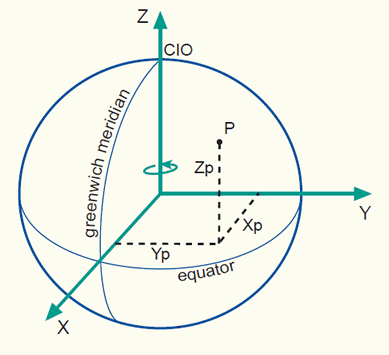
\includegraphics[width=0.7\textwidth]{coord_geocentric}
            \caption{Sistema de coordenadas Geocéntricas}
            \label{fig:coord_geocentric}
            \caption*{Fuente: \cite{coords2009} }
          \end{center}
        \end{figure}

        Este sistema de coordenadas no es muy usado en la representación de datos, pero a veces se lo requiere para análisis de algoritmos y geometría computacional.
      % subsection coordenadas_geocentricas (end)

      \subsection{Coordenadas Geográficas} % (fold)
      \label{sub:coordenadas_geograficas}
        El sistema de coordenadas Geográficas, ver figura \ref{fig:coord_geographic}, utiliza las coordenadas angulares latitud  (\emph{phi} o ${\phi}$) y longitud (\emph{lambda} o ${\lambda}$). Este sistema de coordenadas se expresa en grados, se lo puede representar con la forma \emph{grados:minutos:segundos }\verb|(17° 23' 37.4226" S, 66° 8' 44.691" W)|, o de la forma más común \emph{grados decimales} \verb|(-66.1457475 S, -17.3937285 W)|. \\

  Dentro de ese sistema de coordendas, esta el que es el más ampliamente usado y el que usan por defecto los sistemas \emph{GPS}, es el denominado ``WGS 84'' (\emph{World Geodetic System 1984}) y es el que generalmente la mayoría de las aplicaciones usan para el manejo de mapas. Es el sistema que maneja los más ampliamente conocidos ``latitud y longitud''.\\

        \begin{figure}[H]
          \begin{center}
            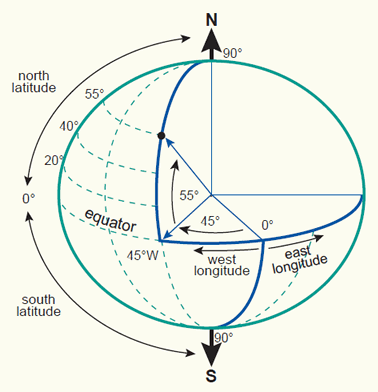
\includegraphics[width=0.7\textwidth]{coord_geographic}
            \caption{Sistema de coordenadas Geográficos}
            \label{fig:coord_geographic}
            \caption*{Fuente: \cite{coords2009} }
          \end{center}
        \end{figure}




      % subsection coordenadas_geograficas (end)

      \subsection{Coordenadas Proyectadas} % (fold)
      \label{sub:coordenadas_proyectadas}
        Un sistema de coordenadas proyectadas es una representación plana y bidimensional de la  tierra. Se basa en un sistema de coordenadas \emph{geográficas esféricas}, pero utiliza unidades de \emph{medida lineales} para las coordenadas, de forma que los cálculos de distancia y área se pueden realizar en términos de esas mismas unidades. \cite{projected}

        Un sistema de coordenadas proyectadas requiere tomar la superficie esférica de la tierra y ``aplanarla'', este procedimiento se lo realiza con la finalidad de tener un mapa representable en una hoja de papel así como en la pantalla de la computadora. Sin embargo este procedimiento introduce diversos tipos de distorsión por lo que existen diferentes clases de proyecciones que varían según la región de la Tierra que se quiere representar.

        La proyección que usan por ejemplo, \emph{Google Maps} y \emph{Open Street Maps} es la \emph{Mercator Projection}, esta proyección está diseñada para preservar los ángulos y las formas de las líneas en forma recta, pero distorsiona los tamaños y las distancias mientras más lejos se encuentran de la línea del Ecuador. Esta proyección se puede apreciar en la figura \ref{fig:mercator_proyection}. \cite{gmaps_osm}

% Google Maps usa la Proyección de Mercator para mostrar su mapa

        \begin{figure}[H]
          \begin{center}
            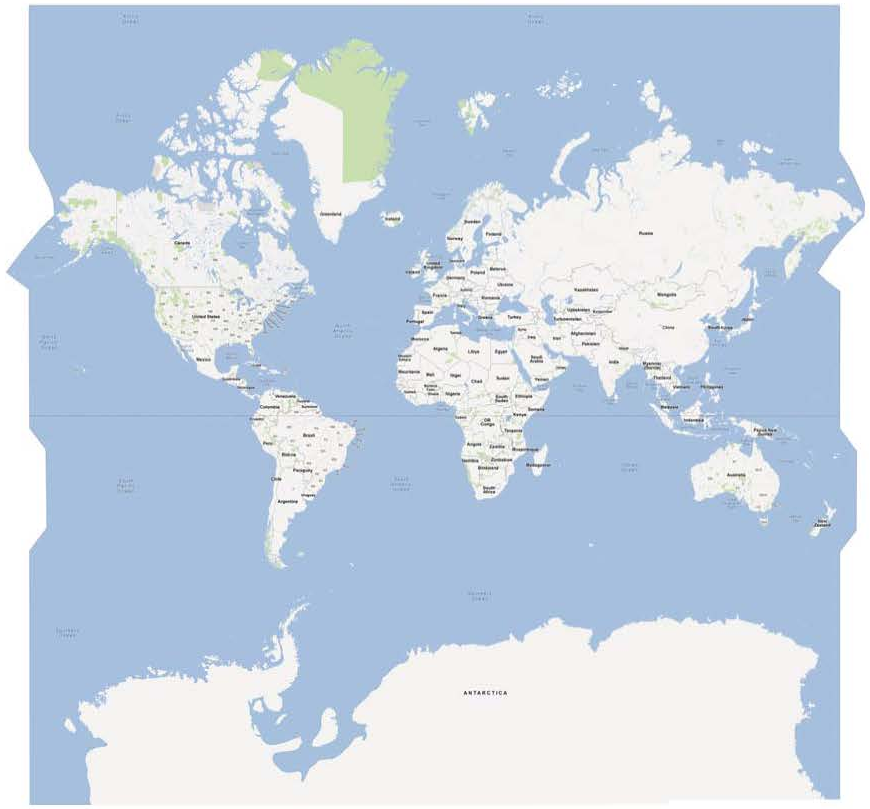
\includegraphics[width=0.6\textwidth]{mercator_proyection}
          \end{center}
          \caption{Sistema de coordenadas Proyectadas}
          \label{fig:mercator_proyection}
          \caption*{Fuente: \cite{coords2009} }
        \end{figure}

        Tal como se puede apreciar en la figura \ref{fig:mercator_proyection}, la distorsión de esta proyección se hace evidente si se observa la zona de Groenlandia ya que parecería tan grande como África o América del Sur, cosa que no es cierta, ya que Groenlandia es casi 14 veces más pequeño que África. A pesar de esta distorsión tan marcada, la \emph{Proyección de Mercator} es una de las más usadas.
         % de hecho Google Maps usa esta proyección.
      % subsection coordenadas_proyectadas (end)

  %
  %     \section{Que se usó en la Aplicación} % (fold)
  %     \label{sec:que_se_uso_en_la_aplicacion}
  %       Es importante entender las diferencias entre los distintos tipos de sistemas de coordenadas porque computacionalmente realizar operaciones sobre los sistemas de coordenadas tiene un costo.
  %       Si se usara el sistema de coordenadas geográfico (WSG84) este es el más apropiado si se necesitaría usar grandes extensiones de la superficie terrestre, que al ser una estructura elipsoidal el costo computacional para realizar las operaciones matemáticas de calcular distancias, intersecciones, etc. es más elevado. En cambio el uso de un sistema de coordenadas proyectado (Mercator Projection) tiene un costo computacional más bajo, ya que se estaría trabajando con un sistema geométrico.\\
  %
  %       % Por otro lado,
  %       También hay tomar en cuenta la base de datos, ya que será esta la que se encargará de manejar los datos espaciales. Al estar usando PostGIS, se puede ver que en su documentacion\footnote{ http://postgis.org/documentation/manual-1.5/ch04.html} que claramente exorta el uso de un sistema geometrico sobre el uso de un sistema geografico si  se va trabajar con datos que cubran una pequena area geografica. Tomando en cuenta esta recomendación y el tamaño del área de estudio (el campus de la UMSS), se procedió a implementar en la base de datos el uso de la proyección Mercator. Se va usar Mercator sobre las otras proyecciones porque aparte de las ventajas que se mencionaron con anterioridad, Google Maps usa esta proyección y ya que se usará este mapa lo más correcto es trabajar con la misma proyección.
  %
  %
  %       % Comoprojected
  %       % PostGIS maneja dos tipos de datos, geográficos y geométricos
  %
  %     % section que_se_uso_en_la_aplicacion (end)
  % % section sistema_de_coordenadas_para_datos_geograficos (end)
  % % \section{Tipo de archivos} % (fold)
  % % \label{sec:tipo_de_archivos}
  % %
  % % section tipo_de_archivos (end)
  %
  % \section{Implementación} % (fold)
  % \label{sec:Implementacion}
  %   Para manejar datos georreferenciados con tecnología JavaScript, ya que se implementó el Backend con NodeJS, se hizo uso de la librería \textbf{KnexJS} para manejar la conexión a la base de datos PostgreSQL, y BookshelfJS para las consultas SQL pero para las consultas con datos geospaciales se realizó a través de esta herramienta pero usando la forma \emph{Raw SQL}\footnote{Raw SQL se refiere a consultas en ``SQL puro'' ya que el fuerte de BookshelfJS es el manejo de las consultas en forma de objetos (ORM), lamentablemente actualmente no existe mucho soporte para manejar datos geoespaciales}.
  %
  %   \begin{center}
  %     \begin{verbatim}
  %       var raw = "SELECT " +
  %                   " ST_AsGeoJSON(geom)::json As geometry," +
  %                   " name," +
  %                   " description," +
  %                   " phone," +
  %                   " level," +
  %                   " gid As id " +
  %                 " FROM place WHERE LOWER(name)
  %                        like LOWER('%" + name + "%')";
  %     \end{verbatim}
  %   \end{center}
  %
  %   De esta forma es que se recupera de la base de datos un lugar georreferenciado, donde este tiene un nombre, una descripción, un teléfono, el nivel o piso donde se encuentra pero lo importante de esta consulta es la obtención del ``punto'' geoespacial del lugar.
  %
  %   \begin{center}
  %     \begin{verbatim}
  %       "POINT (-66.14857015827988 -17.394421906929086)"
  %     \end{verbatim}
  %   \end{center}
  %
  %   % var raw = "SELECT seq, id1 AS node, id2 AS edge, cost
  %   %            FROM pgr_dijkstra('SELECT gid AS id,
  %   %                                     source::integer,
  %   %                                     target::integer,
  %   %                                     st_length(geom) AS cost
  %   %                               FROM public.ways', targetId, sourceId, false, false);";
  %
  %
  %    Este atributo es de tipo \emph{punto} o \emph{point} el cual tiene un \emph{SRID}\footnote{ Spatial Reference System Identifier, El \emph{SRID} corresponde a un sistema de referencia espacial basado en el elipsoide concreto usado para la creación de mapas de tierra plana o de tierra redonda.\cite{msdn_srid} } \emph{3857}\footnote{La proyección Mercator usa el EPSG 3857}, el SRID  es la llave primaria de la tabla \emph{spatial\_ref\_sys} que se crea cuando se inicializa una base de datos que soporte informacion geoespacial (PostGis), esta tabla provee la información necesaria para interpretar y convertir correctamente todas las coordenadas existentes, el \emph{SRID 3857} está definida en la tabla \emph{spatial\_ref\_sys} como ``Popular Visualisation CRS / Mercator''.\\
  %
  %
  %   Obtener la coordenada es el primer paso, seguidamente se debe mostrarlo sobre un mapa, en este caso \emph{Open Street Maps}, como se puede apreciar en la figura \ref{fig:ember_leaflet}, esta interfaz está implementada usando \emph{ember-leaflet}, el cual está principalmente diseñada para ofrecer una mejor experiencia de usuario en celulares smartphones.\\
  %
  %   % \begin{center}
  %   %   \begin{verbatim}
  %   %     var maker = new google.maps.Marker({
  %   %       position: new google.maps.LatLng( lat, lng  )
  %   %       map: UMSS.map
  %   %     });
  %   %   \end{verbatim}
  %   % \end{center}
  %
  %   \begin{verbatim}
  %     {{#leaflet-map lat=lat lng=lng zoom=zoom}}
  %       {{tile-layer url="http://{s}.tile.openstreetmap.fr/hot/{z}/{x}/{y}.png" }}
  %         {{#marker-layer location=location}}
  %           <h3>{{model.name}}</h3>
  %           {{model.description}} <br>
  %           <strong>telf:</strong> {{model.phone}} <br>
  %           <strong>piso </strong>#{{model.level}}
  %       {{/marker-layer}}
  %     {{/leaflet-map}}
  %   \end{verbatim}
  %
  %   \begin{figure}[H]
  %         \begin{center}
  %           \caption{\emph{ember-leaflet} nos ayuda a desplegar un mapa y mostrar un \emph{punto} o \emph{lugar} con un \emph{marcador} y dibuja una línea de color rojo sobre el mapa.}
  %           \label{fig:ember_leaflet}
  %           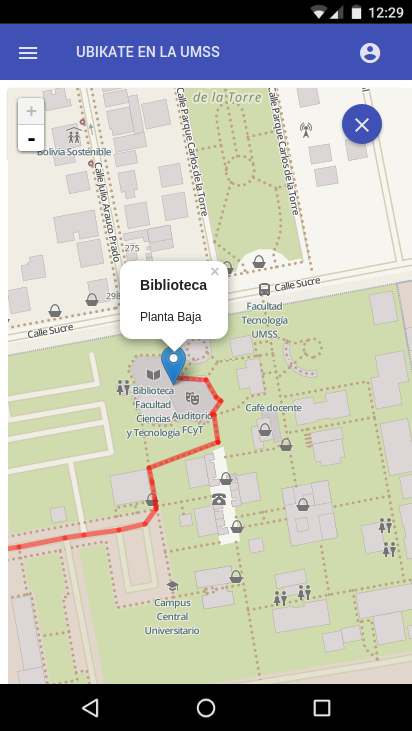
\includegraphics[width=0.5\textwidth]{ember_leaflet}
  %         \end{center}
  %         \caption*{Fuente: Elaboración propia.}
  %   \end{figure}
  %
  %

    % Pero esta coordenada  no sería  fácil de entender sin una adecuada representación sobre un mapa,


  % section Implementacion (end)
  % \section{Los datos} % (fold)
  % \label{sec:los_datos}


  %   Una vez implementada la Base de datos es necesario insertar ``los datos''
  % % section los_datos (end)


  % -------------------------------------------------------------------
  % -------------------------------------------------------------------
% -------------------------------------------------------------------

  % \section{Conclusión} % (fold)
  % \label{sec:geo_conclusion}
  %
    %
    % Los Mapas son herramientas muy útiles a la hora de desplegar información, pero realizar el mapa, crear las fórmulas matemáticas con las cuales se trabajará, determinar cómo se usarán estas fórmulas para una representación adecuada de la superficie terrestre, es una tarea muy compleja. Como programador la tarea más complicada fue determinar el tipo de mapa y el sistema de coordenadas más adecuado para el tipo proyecto que se necesita desarrollar.\\
    %
    % Los términos de longitud y latitud son en un inicio, más fácilmente comprendidos que un sistema proyectado, pero no se puede tomar a la ligera una correcta comprensión del uso de los \emph{sistemas de coordenadas} en una base de datos espacial, un mal uso de estos conceptos puede generar errores a la hora de manejar datos  espaciales o en el resultado de las operaciones sobre estos  datos, llegando a resultados no deseados y que pueden costar más tiempo y dinero en una posterior corrección.\\
    %
    %
    % Para dibujar líneas rectas sobre un mapa hay que tomar en consideración que la tierra no es plana y las líneas que en un mapa parecen líneas rectas, realmente no son rectas, ya que el planeta Tierra es un \emph{esferoide oblato} por lo que las líneas en apariencia rectas tienen la curvatura natural del planeta Tierra. En distancias largas se nota mucho mas la utilidad de usar mapas con \emph{sistemas proyectados}, pero también es cierto que para una área pequeña como es el campus de la Universidad de San Simón este problema no tiene un gran impacto pero no está demás en tomar en cuenta esta característica en el análisis de datos geoespaciales, tomando en cuenta estas caracteristacas de la Geolocalizacion se llego a la conclucion de usar
    % el sistema de \emph{coordenadas projectadas}, mas especificamente la proyección \emph{SRID 3857}.\\
    %
    %
    %
    % La geolocalización es actualmente una tecnología y una herramienta usada en gran medida por una gran cantidad de aplicaciones web, añadiendo búsquedas y resultados personalizados a nivel país, ciudad, barrio y calle, resultando en una gran variedad de servicios y que actualmente es de gran ayuda en diferentes escenarios. La geolocalización ayuda a moverse por una ciudad, encontrar restaurantes, cines, transporte, etc. actualmente es una de las herramientas mas usadas y desarrolladas a nivel de industria, comercio, turismo, etc. y vale la pena estudiarla y entenderla.\\
    %
    %
    %





% ************************************************************
    % Maps are deceivingly simple tools, and cartography a surprisingly complex discipline. While the most trouble many of us will have with a map is figuring out how to fold it, this simplicity belies great sophistication that has been developed over the years.
  % section geo_conclusion (end)


  % \begin{description}
  %   % \item[SIG] Un Sistema de Información Geográfica es una manera de visualizar como es y que está ocurriendo en algún lugar. La posibilidad de incorporar coordenadas con precisión.

  %   % A GIS is a collection of software, normally manipulated by its user through a single interface, and designed to perform a wide range of operations on geographic data.
  %   % Research  Methods in Geography
  %   % Basil Gomez and John Paul Jones III.
  %   % ISBN 978-1-4051-0710-5

  %   \item[Datum]
  %   \item[]
  %   \item[]
  % \end{description}

  % procesar
  % Se tien
  % , Sistema de Posicionamiento Global por sus siglas en espanol
% chapter geolocalizacion (end)

  % \section{Ruta Óptima} % (fold)
\label{cha:ruta_optima}

En general el mejor camino o el más óptimo para ir de un punto a otro es aquel que toma menos tiempo en ser recorrido, pero para definir que un camino es óptimo hay que tomar en cuenta las características de este, por ejemplo, si se va en coche hay que tomar en cuenta la dirección de las calles, los cruces, etc. si se va caminando hay que ver las características del terreno, caminos cortados, distancias, etc.\\


Encontrar la ruta óptima entre 2 puntos es un problema al cual se enfrentan las personas diariamente, por ejemplo, las empresas de transporte, de correo, etc., necesitan mejorar la eficiencia del trayecto y a la vez reducir el consumo de combustible, para mejorar la atención al cliente y a la vez reducir costos de operación. \\

Dentro el campus Universitario es generalmente prioritario optimizar el tiempo de busqueda de algun lugar o punto de interés al cual se quiera llegar, ya sea como estudiante o visitante externo.\\


Si se analiza el terreno que se va a cubrir con la aplicación, el campus ``Las Cuadras'' de la Universidad Mayor de San Simón ubicado entre las calles Oquendo, Sucre,  Belzu y M. U. López, se tiene que el camino óptimo es siempre el más corto o de menor longitud, el método de desplazamiento que se tomara en cuenta será \emph{caminando}, el terreno es llano y la única restricción es respetar las rutas peatonales.\\

% El problema de la ruta más corta es ampliamente usado por las empresas de transporte, correos, etc., que necesitan mejorar la eficiencia del trayecto y a la vez reducir el consumo de combustible, dentro del campus universitario, reducir el tiempo en el cual encontramos un aula o una oficina mejoraría en gran medida la presentación de la Universidad hacia gente externa que necesitan hacer uso o encontrar algún lugar en especifico ya que lamentablemente esta información actualmente sólo te la pueden ofrecer las personas que conocen el lugar de antemano y aun en esos casos existe la posibilidad de no encontrar el lugar que se está buscando.\\
% La resolución de este problema es la se analizará en este capítulo.

El presente problema se lo podría definir como, encontrar la ruta más corta de un punto a otro punto, donde los puntos están interconectados por una red de caminos. El problema descrito se lo puede resolver y describir como un caso específico de la teoría de grafos.



  \subsection{Grafos} % (fold)
  \label{sec:teoria_grafos}


    % \section{Definiciones} % (fold)
    % \label{sec:grafos_definiciones}
      Inicialmente es necesario aclararar algunos términos usados en la teoría de grafos.

      % El grafo que es la reprentacion

      % \begin{description}
      %   \item[Grafo] Un grafo G consiste en un conjunto  vértices V y un conjunto de aristas A, y se lo escribe como G(V,E).
      %   \item[Vertice]
      % \end{description}

      \begin{itemize}
        \item \textbf{Grafo:} Un \emph{grafo} $G$ consiste en un conjunto de vértices $V$ y un conjunto de aristas $A$, y se lo representa con $G(V,A)$.

        \item  \textbf{Vértice:} El \emph{vértice} \emph{v} es adyacente a \emph{u}, o a un vecino de \emph{u}, si y sólo si $(u,v) \in A$. Los vértices también son llamados nodos.

        \item  \textbf{Arista:}
        Cada \emph{arista} o arco es representada por un par de elementos $(u,v)$, donde los elementos $u,v \in V$, son los nodos que une la arista.

        % Para fines prácticos, no  consideraremos las aristas de la forma (u,u)

        \item \textbf{Grafo no Dirigido:}
        En un \emph{grafo no dirigido} $G$, dos vértices $u$ y $v$ se dice que están conectados si hay un camino en $G$ de $u$ a $v$ (y cómo $G$ no es dirigido, también hay un camino de $v$ a $u$). Un grafo  se denomina completo si para todos los pares $u,v \in V$ existe una arista $(u,v) \in A$.

        % En un \emph{grafo no dirigido}, dado una arista $(u,v)$, $v$ es adyacente de $u$, y simétricamente \emph{u} es adyacente de \emph{v} y si el par de vértices que representan la arista no tiene orden, por lo tanto la arista $(u,v)$ y $(v,u)$ representa la misma arista.

        \item \textbf{Grafo Dirigido:} En cambio en un \emph{grafo dirigido} las aristas $(u,v)$ y $(v,u)$ representan dos diferentes aristas. También se puede anotar un tercer componente, llamado peso o costo, en ese caso estaríamos hablando de un \emph{grafo ponderado}.

        % Un camino en un grafo es una secuencia de nodos $v_{1}$, $v_{2}$, \ldots{}, $v_n$ tal que $(v_{1}, v_{2}), (v_{2}, v_{3}), \ldots{}, (v_{n-1}, v_n)$ son aristas.
        %
      \end{itemize}



    % \end{description}
    % subsection grafos_definiciones (end)
    % \subsection{Representacion de un Grafo} % (fold)
    % \label{sec:representacion_de_un_grafo}
      Existen diversas formas de representar un grafo sea dirigido o no-dirigido, pero entre las mas usadas están la matriz de adyacencias y la lista de adyacencias.

      \subsection{Matriz de adyacencias de un Grafo} % (fold)
      \label{sub:matriz_de_adyacencias_de_un_grafo}
        Sea $G = (V,A)$ un grafo de \emph{n} vértices. La matriz de adyacencias $M$  para $G$ es una matriz $M_{nxn}$ de valores booleanos, donde $M(i,j)$ es verdad si y sólo si existe un arco desde el nodo \emph{i} al nodo \emph{j}.

        \begin{displaymath}
          M(i,j) = \left\{
          \begin{array}{ l l }
            1, & \textrm{si existe la arista } (i,j) \\
            0, & \textrm{en caso contrario}
          \end{array} \right.
        \end{displaymath}


        Las filas y las columnas de la matriz representan los nodos del grafo.
        Cuando el grafo es no-dirigido la matriz de adyacencias es simétrica, como se puede ver en el grafo de la figura \ref{fig:grafo_ponderado} y su correspondiente matriz de adyacencias.
        % El cuadro \ref{tab:matriz} representa la matriz de adyacencias de la figura \ref{fig:grafo_ponderado} representa
        % La matriz de adyacencias, que se puede observar a continuacion, es la  misma matriz de la relación $A$ de $V$ en $V$ porque indica cuales vertices están relacionados o unidos por una arista.


        % \begin{tikzpicture}[->,>=stealth',shorten >=1pt,auto,node distance=3cm,
        %         main node/.style={circle,draw,font=\sffamily\Large\bfseries}]
% !ht
        \begin{figure}[H]
          \begin{center}

            \begin{tikzpicture}[->,>=stealth',shorten>=1pt,auto,node distance=3cm,main node/.style={circle,draw,font=\sffamily\Large\bfseries}]

              \node[main node] (1) {a};
              \node[main node] (2) [below right  of=1] {b};
              \node[main node] (3) [above right of=2] {c};
              \node[main node] (4) [below left of=2] {d};
              \node[main node] (5) [right of=2] {e};
              % \node[main node] (6) [right of=5] {f};
              % \node[main node] (7) [above right of=6] {g};
              % \node[main node] (4) [below right of=1] {d};

              \path[every node/.style={font=\sffamily\small}]
                (1) edge node [auto] {3} (2)
                    edge node[left] {5} (4)
                (2) edge node[left] {8} (3)
                    edge node[right] {4} (4)
                    edge node[auto] {3} (5)
                (3) edge node[left] {7} (5)
                (4) edge node[below] {14} (5);

            \end{tikzpicture}

            \caption{Grafo ponderado no-dirigido}
            \label{fig:grafo_ponderado}
            \caption*{Fuente: Elaboración propia}

          \end{center}
        \end{figure}

        % La matriz de adyacencias, que se puede observar a continuacion, es la  misma matriz de la relación $A$ de $V$ en $V$ porque indica cuales vertices están relacionados o unidos por una arista.


        \begin{table}[H]
          % \label{tab:matriz}
          \begin{center}
            \begin{displaymath}
              M(i,j) =
              \bordermatrix{ ~ & a & b & c & d & e \cr
                             a & 0 & 3 & 0 & 5 & 0 \cr
                             b & 3 & 0 & 8 & 4 & 3 \cr
                             c & 0 & 8 & 0 & 0 & 7 \cr
                             d & 5 & 4 & 0 & 0 & 14\cr
                             e & 0 & 3 & 7 & 14& 0  }
            \end{displaymath}
            \caption*{Matriz de adyacencias del grafo de la figura  \ref{fig:grafo_ponderado}}
          \end{center}
        \end{table}


      % subsubsection matriz_de_adyacencias_de_un_grafo (end)

    % subsection representacion_de_un_grafo (end)
    \subsection{El Problema de la ruta mas corta} % (fold)
    \label{sec:ruta_mas_corta}
      Dados los vértices $v_{i}$ y $v_{j}$ de un grafo $G = (V,A)$ se llama trayectoria mínima o camino minimo  de \(v_i\) a \(v_j\) al numero de aristas del camino de longitud mínima que va desde $v_i$ a $v_j$ y se representa por $d(v_i, v_j)$.

      Cuando en el grafo no exista un camino de $v_i$ a $v_j$ se dice que el camino minimo es $d(v_i, v_j) = \infty$ \\

      Para determinar el camino mínimo que va desde un único vértice a cualquier otro vértice se puede usar el algoritmo de Dijkstra.



      \subsubsection{Algoritmo de Dijkstra} % (fold)
      \label{sub:algoritmo_de_dijkstra}
      El algoritmo de  Dijkstra fue descrito en 1959 por \emph{Edsger Dijkstra}, y permite encontrar la trayectoria más corta entre dos nodos específicos, cuando los valores de los arcos son todos positivos\\

      El algoritmo asigna un etiqueta a cada nodo en el grafo. Esta etiqueta es la distancia que hay desde el nodo \emph{s} escogido como origen a lo largo de la trayectoria más corta encontrada, hasta el nodo que se está etiquetando.\\

      La etiqueta de cada nodo puede estar en 2 estados:

      \begin{itemize}
        \item[\textbf{a.}] Puede ser permanente; en este caso la distancia encontrada es a lo largo de la trayectoria, la más corta de todas las encontradas.
        \item[\textbf{b.}] Puede ser temporal; cuando hay incertidumbre de que la trayectoria encontrada sea la más corta de todas.
      \end{itemize}

      A medida que el método trabaja se cambian gradualmente las etiquetas temporales por etiquetas permanentes. Al comienzo se tiene un conjunto de nodos con etiquetas temporales y el objetivo es hacer que esas etiquetas disminuyan, encontrando trayectorias a esos nodos usando trayectorias a nodos etiquetados permanentemente. Cuando esto se ha logrado, se selecciona el nodo con la etiqueta temporal más pequeña y esta etiqueta se convierte en permanente. El proceso se repite hasta que al nodo terminal \emph{t} se le haya asignado una etiqueta permanente, pero esto puede ocurrir eventualmente, ya que cada vez que el algoritmo es usado, una de las etiquetas es omitida y así el número de nodos con etiquetas temporales decrece a cero. \cite{teoria_grafos} \\


      % subsection algoritmo_de_dijkstra (end)
    % subsection ruta_mas_corta (end)
  % section teoria_grafos (end)


% ********************************************************************
% ********************************************************************
% ********************************************************************

  % \subsection{Conclusi\'on} % (fold)
  % \label{sub:ruta_conclusion}


    % ********************************************************************
    % ********************************************************************
% ********************************************************************

  % section ruta_conclusion (end)
% chapter ruta_optima (end)


  % Algoritmos de busqueda de caminos - ruta corta

  % Como determino que tipo de grafo tengo


  % % \section{La Red} % (fold)
  % % \label{sec:la_red}

  % % % section la_red (end)

  % \section{Algoritmo} % (fold)
  % \label{sec:algoritmo}

  % % section algoritmo (end)

  % \section{Algoritmo de Dijkstra} % (fold)
  % \label{sec:algoritmo_de_dijkstra}

  % % section algoritmo_de_dijkstra (end)

  % % Por lo tanto se implementó un grafo no dirigido (sin dirección), el cual se analizará en este capítulo.


  % Un problema de este tipo es represetable como un proble de teoria de grafos.


  % Cuando se tiene que encontrar un camino o ruta optima entre 2 puntos, se tienen que tomar en cuenta varios puntos


  % El problema de encontrar una ruta optima entre 2 puntos se lo puede resolver/representar como problema de grafos


  % Caminos mínimos en grafos

  % Solución voraz: Algoritmo de Dijkstra

  % para grafos dirigidos (la extensión a no dirigidos es inmediata)
  % genera uno a uno los caminos de un nodo v al resto por orden creciente de longitud
  % usa un conjunto de vértices donde, a cada paso, se guardan los nodos para los que ya se sabe el camino mínimo
  % devuelve un vector indexado por vértices: en cada posición w se guarda el coste del camino mínimo que conecta v con w
  % cada vez que se incorpora un nodo a la solución se comprueba si los caminos todavía no definitivos se pueden acortar pasando por él
  % se supone que el camino mínimo de un nodo a sí mismo tiene coste nulo
  % un valor en la posición w del vector indica que no hay ningún camino desde v a w
  % E.W. Dijkstra:
  % “A note on two problems in connexion with graphs”,
  % Numerical Mathematica, 1, pp. 269-271, 1959.

  %
% \subsubsection{Implementar módulo para añadir lugares al sistema}
\subsubsection{Registro de Lugares en el sistema}

Para registrar un \emph{lugar} primeramente se implementó el formulario que se usará para recolectar la información del \emph{lugar}, el formulario fue creado usando \emph{EmberJs} y se lo puede ver en la figura \ref{fig:new_place}. \\

\begin{figure}[H]
     \begin{center}
       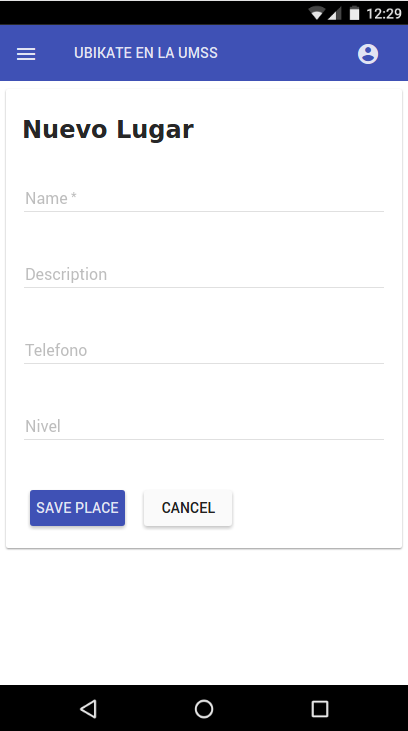
\includegraphics[width=0.3\textwidth]{new_place}

       \caption{Formulario para añadir un nuevo \emph{lugar}.}
       \label{fig:new_place}
       \caption*{Fuente: Elaboración propia.}
     \end{center}
\end{figure}

Posteriormente es necesario crear la petición HTTP desde el controlador de \emph{EmberJS} hacia el API, en el cuerpo de la petición se incluye la posición georeferenciada del celular utilizando el API de Geolocalización de HTML5 usada anteriormente para encontrar la ubicación del usuario, también se incluye el nombre, la descripción, el teléfono y el nivel del \emph{lugar}. En el codigo \ref{new_place_request} se puede ver la implementación de la petición.


% En la figura \ref{fig:new_place} se puede ver el formulario implementado usando \emph{ember-paper}, el cual colecciona los datos que se quieren introducir y se los envía al backend usando una llamada AJAX, como se puede ver en el siguiente código, para crear la petición POST se obtiene las coordenadas actuales del dispositivo móvil además de los datos recolectados del formulario y que con la ayuda de \emph{JQuery} es enviado al API el cual maneja la información recibida y se encarga de insertar los datos en la base de datos.\\

% \newpage
\begin{center}
 \begin{lstlisting}[label=new_place_request,caption=POST request creado en el controlador de \emph{ember}]

   var payload = {
       name: nombre,
       description: descripcion,
       phone: telefono,
       level: nivel,
       lat: latitud,
       lon: longitud
   };

   var url = (ENV.APP.API_HOST || '') + '/api/v1/places/';
   jQuery.post(url, payload).then(
       function(data) {
           var transition = controller.get('transition');
           if (transition) {
               self.transitionTo('places.show');
           } else {
               self.transitionTo('places');
           }
       },
       function(error) {
           controller.set('message', error.responseText);
       }
   );

 \end{lstlisting}
\end{center}

% En esta iteración se implementó la opción de añadir más lugares al sistema, de editarlos y eliminarlos, y la primera tarea es crear las consultas SQL para llevar a cabo las tareas. \\

% por lo que es necesario crear las consultas SQL que insertaran los datos enviados desde el dispositivo móvil al servidor. \\

% Como requisito para insertar un nuevo ``lugar'', se requiere que el usuario esté posicionado en el ``lugar'' ya que se usaran sus coordenadas para posicionar el ``lugar''. Las coordenadas del usuario son obtenidas usando el API de Geolocalización propia de HTML5, usada anteriormente para encontrar la ubicación del usuario \emph{visitante} en la iteración 2.\\

% Posteriormente se necesita implementar el formulario que el usuario usará para insertar los datos del ``lugar'': el nombre, la descripción, el teléfono y el nivel.\\

% Para insertar un ``lugar''  en la base de datos se usó el codigo \ref{new_place}, donde se puede observar la consulta SQL usada, para la cual se necesita capturar la latitud y longitud respectiva donde se encuentra el usuario, además de los datos del ``lugar''.\\

La petición creada es recibida en el API utilizando el \emph{endpoint} RESTful designado para ello, \verb|router.post('/', places.newPlace);|, el \emph{endpoint} se encarga de mandar la información recibida hacia la base de de datos, tomando en cuenta que la posición del lugar es un tipo especial de la base de datos, la latitud y longitud necesitan ser transformadas al momento de insertar el \emph{lugar} en la base de datos, como se muestra en el codigo \ref{cod-new_place_api}.


\begin{center}
 \begin{lstlisting}[label=cod-new_place_api,caption=Insertar un ``lugar'' en la base de datos.]

   router.post('/', places.newPlace);

   var newPlace = (req, res) => {
       var name = req.body.name || '';
       var lat = req.body.lat || '';
       var lon = req.body.lon || '';
       var description = req.body.description || '';
       var phone = req.body.phone || '';
       var level = req.body.level || '';

       let raw = `insert into place (name, geom, description, phone, level)
                  values ('${name}',
                          ST_GeomFromText('POINT(${lon} ${lat})', 3875),
                          '${description}',
                          '${phone}',
                          '${level}'
                         );`;

       Knex.raw(raw)
           .then(function(data) {
               res.json({
                   "message": "Place saved successfully!",
                   "data": data
               });
           })
           .catch(function(error) {
               res.send("Error:", error);
           });
   };

 \end{lstlisting}
\end{center}




% Para la creación de un ``lugar'' es necesario implementar un \emph{endpoint} en el API y siguiendo las convenciones REST se , para que como ya se explicó anteriormente el frontend pueda comunicarse con el backend. \\

% En el API de la aplicación, se implementó un \emph{endpoint} para que pueda manejar los \emph{request} del cliente para añadir un lugar, este \emph{request} es enviado usando el verbo HTTP \emph{POST}, que como ya se explicó es el usado en un REST API para crear objetos. \\

\subsubsection{Edición de la información del Lugar}

Para editar de la información de un lugar se rehusó el formulario ya creado para el registro del mismo, pero populando los campos con la información actual del lugar, el resultado se lo puede ver en la figura \ref{fig:place_edit_form}. \\

\begin{figure}[H]
     \begin{center}
       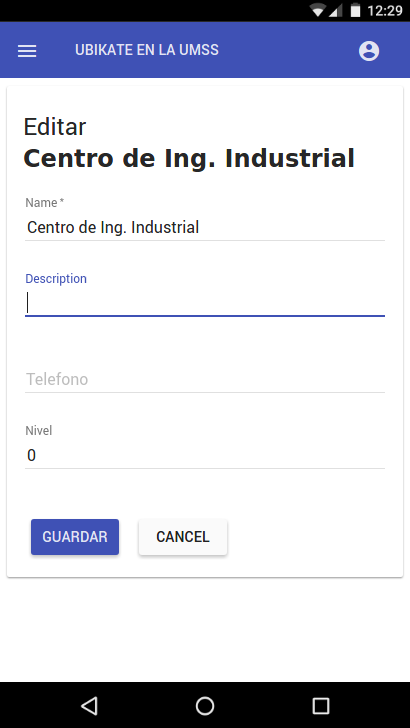
\includegraphics[width=0.3\textwidth]{place_edit_form}

       \caption{Formulario para editar un \emph{lugar}}
       \label{fig:place_edit_form}
       \caption*{Fuente: Elaboración propia.}
     \end{center}
\end{figure}


Los cambios a la información del \emph{lugar} son enviados al API mediante una petición PUT, siguiendo los lineamientos del REST API implementado, esta petición se puede ver en el codigo \ref{cod-edit_place_request}.

% \newpage
\begin{center}
 \begin{lstlisting}[label=cod-edit_place_request,caption=Petición HTTP para editar un lugar.]

   router.put('/:id', places.editPlace);

   var body = {
       name: name,
       description: description,
       phone: phone,
       level: level
   };

   var url = (ENV.APP.API_HOST || '') + `/api/v1/places/${id}`;
   jQuery.ajax({
       url: url,
       type: 'put',
       data: body
   }).then(
       function(data) {
           self.transitionTo('places.show', id);
       },
       function(error) {
           controller.set('message', error.responseText);
       }
   );

 \end{lstlisting}
\end{center}

A diferencia del registro del \emph{lugar}, que guarda la posición georeferenciada al momento de registrar el \emph{lugar}, en la edición de los datos no se está tomando en cuenta este dato porque se noto que generalmente cuando se requiere actualizar los datos del \emph{lugar}, el usuario no se encuentra en la posición original del \emph{lugar} y este dato se pierde, corrompiendo la base de datos. Es por esta razón que se decidió que no se actualizará la posición geográfica del \emph{lugar} sin alguna opción explícita que advierta al usuario de las consecuencias de esta acción, pero como tal tarea no se halla dentro de la \emph{historia de usuario} que se esta implementado, se tomo la decisión de realizarla en una futura iteración.








% \subsubsection{Eliminar un lugar}

% Una vez implementado la lógica para añadir un ``lugar'', se implementó los módulos para poder eliminar el ``lugar'', para esto se añadió un botón en la lista de lugares, el cual despliega un mensaje de advertencia al usuario de que está por eliminar un ``lugar'' y que la acción es irreversible, por lo tanto este botón sólo está disponible para un usuario \emph{administrador}. \\
%
% La verbo  HTTP \emph{DELETE} es el que de acuerdo a la implementación del API REST es el adecuado para eliminar un lugar, por lo tanto es el que se usó en la aplicación. En el codigo \ref{delete_place_enpoint} se puede observar el \emph{endpoint} implementado en el API que se encarga de manejar las peticiones \emph{DELETE} creando una consulta SQL que elimina el lugar de la base de datos.\\
%
% \begin{center}
%   \begin{lstlisting}[label=delete_place_enpoint,caption=DELETE request elimina un lugar.]
%
%     router.delete('/:id', places.deletePlace);
%
%     var deletePlace = (req, res) => {
%         var id = req.params.id;
%
%         Place.forge({
%             gid: id
%         })
%         .destroy()
%         .then(function(model) {
%             res.json({
%                 "message": "Place deleted successfully!"
%             });
%         })
%         .catch(function(err) {
%             res.status(500);
%         });
%     };
%
%   \end{lstlisting}
% \end{center}
%
% En el anterior codigo se puede apreciar la bondad de usar un manejador de bases de datos como \emph{Bookshelf} ya que usando el método \verb|destroy()|, se encarga automáticamente de crear la consulta SQL para eliminar una tupla de la base de datos.\\

  % \begin{table}[H]
  \begin{center}
    \begin{tabularx}{0.75\textwidth}{ X }
      \toprule
      \textbf{Codigo:} CP004
      \makebox[3cm][r]{}
      \makebox[6cm][r]{\textbf{Historia de Usuario:} US03} \\

      \addlinespace
      \textbf{Nombre:} Verificar el marcador del lugar sobre el mapa del campus Universitario. \\

      \addlinespace
      \textbf{Descripción:} Validar que un usuario puede ver un marcador sobre el mapa indicando la posición del lugar dentro del campus Universitario cuando se pide la ruta óptima al lugar. \\

      \addlinespace
      \textbf{Condiciones de Ejecución:}
      Registrar un lugar dentro del campus Universitario. \\

      \addlinespace
      \textbf{Entradas / Pasos de Ejecución:}  \\
      \tab \textbf{1.} Seleccionar el menú \emph{Lugares}. \\
      \tab \textbf{2.} Buscar el lugar registrado.\\
      \tab \textbf{3.} Seleccionar la opción para buscar la ruta al lugar. \\


      \addlinespace
      \textbf{Resultado Esperado:} Una vista del mapa del campus Universitario debe ser desplegado con un marcador sobre la posición del lugar en el centro de la pantalla.  \\

      \addlinespace
      \textbf{Evaluación de la Prueba:} Prueba exitosa. \\

      \bottomrule
    \end{tabularx}
    \caption{Prueba de Aceptación - CP004}
    \label{tab:CP004}
  \end{center}
\end{table}

\begin{table}[H]
  \begin{center}
    \begin{tabularx}{0.75\textwidth}{ X }
      \toprule
      \textbf{Codigo:} CP005
      \makebox[3cm][r]{}
      \makebox[6cm][r]{\textbf{Historia de Usuario:} US04} \\

      \addlinespace
      \textbf{Nombre:} Verificar que una línea roja muestra la ruta óptima hacia el lugar. \\

      \addlinespace
      \textbf{Descripción:} Validar que el usuario puede ver un una línea roja mostrando la ruta óptima entre la posición del usuario y el lugar. \\

      \addlinespace
      \textbf{Condiciones de Ejecución:}
      Registrar un lugar dentro del campus Universitario. \\

      \addlinespace
      \textbf{Entradas / Pasos de Ejecución:}  \\
      \tab \textbf{1.} Seleccionar el menú \emph{Lugares}. \\
      \tab \textbf{2.} Buscar el lugar registrado.\\
      \tab \textbf{3.} Seleccionar la opción para buscar la ruta al lugar. \\


      \addlinespace
      \textbf{Resultado Esperado:} Una vista del mapa del campus Universitario debe ser desplegado con una línea roja uniendo el marcador sobre la posición del usuario y la posición del lugar.  \\

      \addlinespace
      \textbf{Evaluación de la Prueba:} Prueba exitosa. \\

      \bottomrule
    \end{tabularx}
    \caption{Prueba de Aceptación - CP005}
    \label{tab:CP005}
  \end{center}
\end{table}


\backmatter{}
  \begin{thebibliography}{99}
  \bibitem{why_scrum} https://www.scrumalliance.org/why-scrum
  \bibitem{awdr4e} Sam Ruby, Dave Thomas, David Heinemeier Hansson, \emph{Agile Web Development with Rails, Fourth Edition}
  \bibitem{web2}  http://trends.builtwith.com/topsites/Ruby-on-Rails
  \bibitem{web3} tumblr.yasulab.jp/post/10271634919/5-question-interview-with-twitter-developer-alex-payne
  \bibitem{web4} http://www.artima.com/scalazine/articles/twitter\_on\_scala.html
  \bibitem{web5} http://oreilly.com/web2/archive/what-is-web-20.html
  \bibitem{web9} http://radar.oreilly.com/2006/12/web-20-compact-definition-tryi.html
  \bibitem{web6} http://www.ics.uci.edu/~fielding/pubs/dissertation/top.htm
  \bibitem{web7} http://st-www.cs.illinois.edu/users/smarch/st-docs/mvc.html
  \bibitem{web8} http://msdn.microsoft.com/en-us/architecture/bb906060.aspx
  \bibitem{json} http://www.json.org/json-es.html
  \bibitem{coords} http://kartoweb.itc.nl/geometrics/Coordinate\%20systems/coordsys.html
  \bibitem{p_iscs} Introduction to Spatial Coordinate Systems: Flat Maps for a Round Planet,\\ http://msdn.microsoft.com/en-us/library/cc749633(v=sql.100).aspx
  \bibitem{projected_ibm} http://publib.boulder.ibm.com/infocenter/db2luw/v8/index.jsp?\\topic=/com.ibm.db2.udb.doc/opt/csb3022b.htm
  \bibitem{msdn_srid} http://msdn.microsoft.com/es-es/library/bb964707.aspx
  \bibitem{teoria_grafos} Introducción a la Teoría De Grafos, Alfredo Caicedo Barrero, \\ISBN: 978-958-99325-7-5



\end{thebibliography}

  % \listoffigures
  % \listoftables
% \newpage
\end{document}
